\documentclass{article}

\usepackage{hyperref}
\hypersetup{
	colorlinks=true,
	linkcolor=blue,
	urlcolor=cyan,}
\usepackage{booktabs}
\usepackage{textgreek}

%%%%%%%%%%%%%%%%%%%%%%%%%%%%%%%%%%%%%%%%%
% Lachaise Assignment
% Structure Specification File
% Version 1.0 (26/6/2018)
%
% This template originates from:
% http://www.LaTeXTemplates.com
%
% Authors:
% Marion Lachaise & François Févotte
% Vel (vel@LaTeXTemplates.com)
%
% License:
% CC BY-NC-SA 3.0 (http://creativecommons.org/licenses/by-nc-sa/3.0/)
% 
%%%%%%%%%%%%%%%%%%%%%%%%%%%%%%%%%%%%%%%%%

%----------------------------------------------------------------------------------------
%	PACKAGES AND OTHER DOCUMENT CONFIGURATIONS
%----------------------------------------------------------------------------------------

\usepackage{amsmath,amsfonts,stmaryrd,amssymb} % Math packages

\usepackage{enumerate} % Custom item numbers for enumerations

\usepackage[ruled]{algorithm2e} % Algorithms

\usepackage[framemethod=tikz]{mdframed} % Allows defining custom boxed/framed environments

\usepackage{listings} % File listings, with syntax highlighting
\lstset{
	basicstyle=\ttfamily, % Typeset listings in monospace font
}

%----------------------------------------------------------------------------------------
%	DOCUMENT MARGINS
%----------------------------------------------------------------------------------------

\usepackage{geometry} % Required for adjusting page dimensions and margins

\geometry{
	paper=a4paper, % Paper size, change to letterpaper for US letter size
	top=2.5cm, % Top margin
	bottom=3cm, % Bottom margin
	left=2.5cm, % Left margin
	right=2.5cm, % Right margin
	headheight=14pt, % Header height
	footskip=1.5cm, % Space from the bottom margin to the baseline of the footer
	headsep=1.2cm, % Space from the top margin to the baseline of the header
	%showframe, % Uncomment to show how the type block is set on the page
}

%----------------------------------------------------------------------------------------
%	FONTS
%----------------------------------------------------------------------------------------

\usepackage[utf8]{inputenc} % Required for inputting international characters
\usepackage[T1]{fontenc} % Output font encoding for international characters

\usepackage{XCharter} % Use the XCharter fonts

%----------------------------------------------------------------------------------------
%	COMMAND LINE ENVIRONMENT
%----------------------------------------------------------------------------------------

% Usage:
% \begin{commandline}
%	\begin{verbatim}
%		$ ls
%		
%		Applications	Desktop	...
%	\end{verbatim}
% \end{commandline}

\mdfdefinestyle{commandline}{
	leftmargin=10pt,
	rightmargin=10pt,
	innerleftmargin=15pt,
	middlelinecolor=black!50!white,
	middlelinewidth=2pt,
	frametitlerule=false,
	backgroundcolor=black!5!white,
	frametitle={Command Line},
	frametitlefont={\normalfont\sffamily\color{white}\hspace{-1em}},
	frametitlebackgroundcolor=black!50!white,
	nobreak,
}

% Define a custom environment for command-line snapshots
\newenvironment{commandline}{
	\medskip
	\begin{mdframed}[style=commandline]
}{
	\end{mdframed}
	\medskip
}

%----------------------------------------------------------------------------------------
%	FILE CONTENTS ENVIRONMENT
%----------------------------------------------------------------------------------------

% Usage:
% \begin{file}[optional filename, defaults to "File"]
%	File contents, for example, with a listings environment
% \end{file}

\mdfdefinestyle{file}{
	innertopmargin=1.6\baselineskip,
	innerbottommargin=0.8\baselineskip,
	topline=false, bottomline=false,
	leftline=false, rightline=false,
	leftmargin=2cm,
	rightmargin=2cm,
	singleextra={%
		\draw[fill=black!10!white](P)++(0,-1.2em)rectangle(P-|O);
		\node[anchor=north west]
		at(P-|O){\ttfamily\mdfilename};
		%
		\def\l{3em}
		\draw(O-|P)++(-\l,0)--++(\l,\l)--(P)--(P-|O)--(O)--cycle;
		\draw(O-|P)++(-\l,0)--++(0,\l)--++(\l,0);
	},
	nobreak,
}

% Define a custom environment for file contents
\newenvironment{file}[1][File]{ % Set the default filename to "File"
	\medskip
	\newcommand{\mdfilename}{#1}
	\begin{mdframed}[style=file]
}{
	\end{mdframed}
	\medskip
}

%----------------------------------------------------------------------------------------
%	NUMBERED QUESTIONS ENVIRONMENT
%----------------------------------------------------------------------------------------

% Usage:
% \begin{question}[optional title]
%	Question contents
% \end{question}

\mdfdefinestyle{question}{
	innertopmargin=1.2\baselineskip,
	innerbottommargin=0.8\baselineskip,
	roundcorner=5pt,
	nobreak,
	singleextra={%
		\draw(P-|O)node[xshift=1em,anchor=west,fill=white,draw,rounded corners=5pt]{%
		Question \theQuestion\questionTitle};
	},
}

\newcounter{Question} % Stores the current question number that gets iterated with each new question

% Define a custom environment for numbered questions
\newenvironment{question}[1][\unskip]{
	\bigskip
	\stepcounter{Question}
	\newcommand{\questionTitle}{~#1}
	\begin{mdframed}[style=question]
}{
	\end{mdframed}
	\medskip
}

%----------------------------------------------------------------------------------------
%	WARNING TEXT ENVIRONMENT
%----------------------------------------------------------------------------------------

% Usage:
% \begin{warn}[optional title, defaults to "Warning:"]
%	Contents
% \end{warn}

\mdfdefinestyle{warning}{
	topline=false, bottomline=false,
	leftline=false, rightline=false,
	nobreak,
	singleextra={%
		\draw(P-|O)++(-0.5em,0)node(tmp1){};
		\draw(P-|O)++(0.5em,0)node(tmp2){};
		\fill[black,rotate around={45:(P-|O)}](tmp1)rectangle(tmp2);
		\node at(P-|O){\color{white}\scriptsize\bf !};
		\draw[very thick](P-|O)++(0,-1em)--(O);%--(O-|P);
	}
}

% Define a custom environment for warning text
\newenvironment{warn}[1][Warning:]{ % Set the default warning to "Warning:"
	\medskip
	\begin{mdframed}[style=warning]
		\noindent{\textbf{#1}}
}{
	\end{mdframed}
}

%----------------------------------------------------------------------------------------
%	INFORMATION ENVIRONMENT
%----------------------------------------------------------------------------------------

% Usage:
% \begin{info}[optional title, defaults to "Info:"]
% 	contents
% 	\end{info}

\mdfdefinestyle{info}{%
	topline=false, bottomline=false,
	leftline=false, rightline=false,
	nobreak,
	singleextra={%
		\fill[black](P-|O)circle[radius=0.4em];
		\node at(P-|O){\color{white}\scriptsize\bf i};
		\draw[very thick](P-|O)++(0,-0.8em)--(O);%--(O-|P);
	}
}

% Define a custom environment for information
\newenvironment{info}[1][Info:]{ % Set the default title to "Info:"
	\medskip
	\begin{mdframed}[style=info]
		\noindent{\textbf{#1}}
}{
	\end{mdframed}
}
 % Include the file specifying the document structure and custom commands

%----------------------------------------------------------------------------------------
%	ASSIGNMENT INFORMATION
%----------------------------------------------------------------------------------------

\title{Week 1: Introduction to BIOPAC}
\author{BIOE 320 Systems Physiology Laboratory} 
\date{}
%----------------------------------------------------------------------------------------

\begin{document}
\large
\maketitle

\section*{Objectives}
\begin{enumerate}
	\item To become familiar with the format of data display in the BIOPAC Student Lab data window
	\item To learn how to position data within the window by using software tools and pull down menus
	\item To learn how to select and use correct measurement tools for extracting information from the data
	\item To learn how to use journal to record measurements and write notes
\end{enumerate}

\section*{Background}
The lab is based on the BIOPAC Student Lab System that allows data acquisition and analysis of a variety of physiological signals. \textbf{Hardware} components include electrodes, input transducers, connecting cables, and the acquisition unit (MP30, MP35, or MP36) shown in Fig. \ref{basic_scheme}. The \textbf{software} used in this lab consists of the BIOPAC Student Lab Lessions and the BIOPAC Student Lab PRO pre-installed on your computer.

\begin{figure}[h]
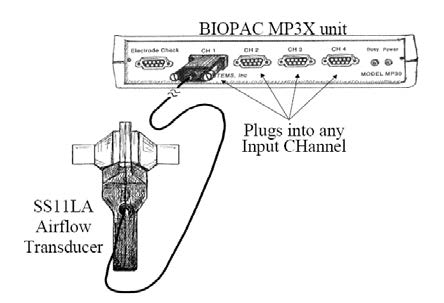
\includegraphics[width=0.5\textwidth]{../images/BIOPAC_1.jpg}
\centering
\caption{Schematic of MP3x acquisition unit and attached transducer}
\label{basic_scheme}
\end{figure}

The lab will introduce you to the BIOPAC system. To complete the in-lab activities, read the instructions carefully and perform each of the steps described in the exercises while answering the questions listed below. 

\begin{info}
	Your knowledge and comfort level in manipulating the data obtained using BIOPAC are critical for success in future labs.
\end{info}

\section*{Getting Started}
Before beginning the lab activity, open the BIOPAC tutorial that can be found in: (need to figure out links)

\begin{enumerate}
	\item Turn on the MP3X acquisition unit by flipping the switch found on the back panel.
		\begin{figure}[h]
		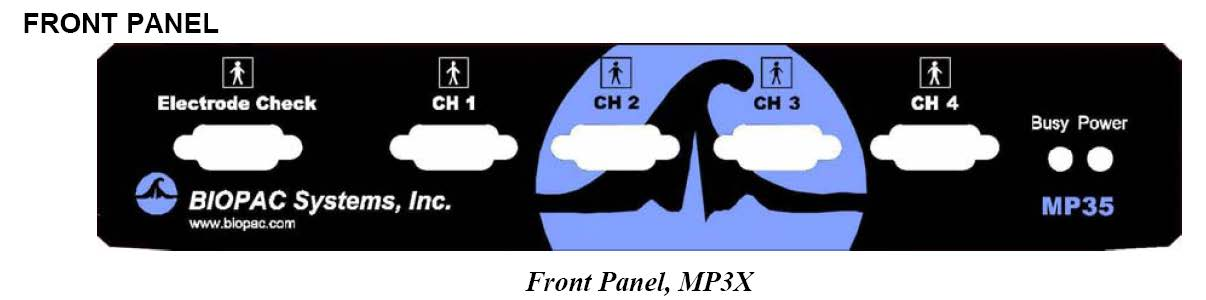
\includegraphics[width=0.8\textwidth]{../images/BIOPAC_2a.jpg}
		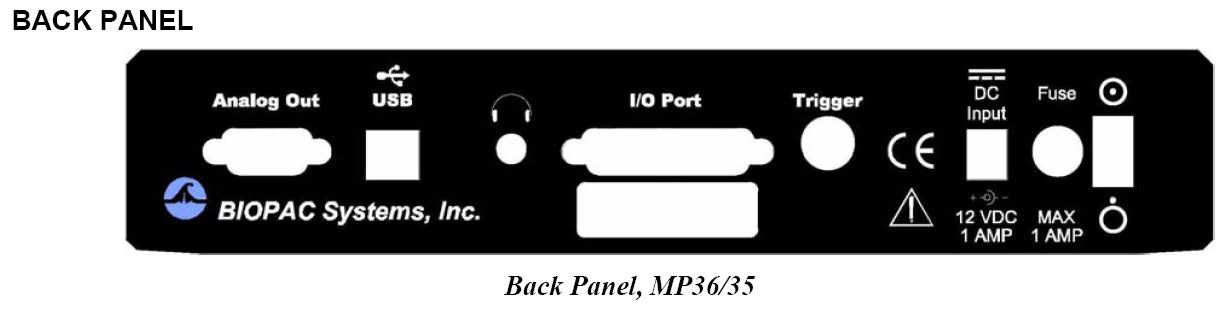
\includegraphics[width=0.8\textwidth]{../images/BIOPAC_2b.jpg}
		\centering
		\caption{MP3X acquisition unit - front panel (top) and back panel (bottom) are shown}
		\label{panels}
		\end{figure}
		
	\item Launch the BIOPAC Student Lab Lessons Software (\textit{Start $\rightarrow$ All Programs $\rightarrow$ BIOPAC Student Lab Lessons 3.7.6})
	
	\begin{warn}
		If you receive the warning prompt shown in Fig. \ref{conn_error}, make sure the acquisition box is on, check the connections to the computer, and restart the hardware and software. If the problem persists, call the instructor or a TA.
	\end{warn}
	
		\begin{figure}[h]
		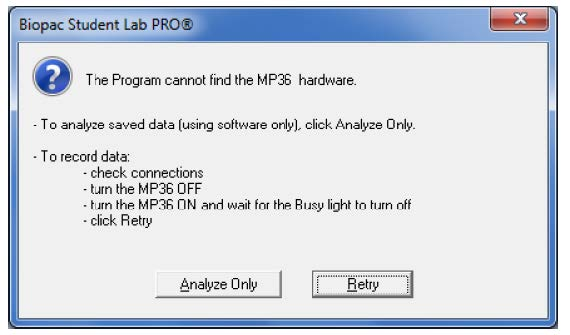
\includegraphics[width=0.8\textwidth]{../images/BIOPAC_3.jpg}
		\centering
		\caption{Connection error prompt}
		\label{conn_error}
		\end{figure}
		
	\item Scroll down the lesson menu to "Review Saved Data," select it, and click OK. A window resembling Fig. \ref{open_data} (left) should appear.
	
		\begin{figure}[h]
		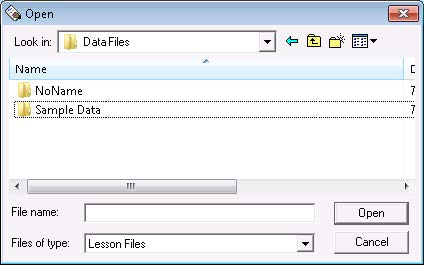
\includegraphics[width=0.4\textwidth]{../images/BIOPAC_4a.jpg}
		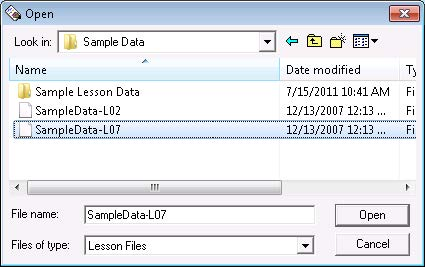
\includegraphics[width=0.4\textwidth]{../images/BIOPAC_4b.jpg}
		\centering
		\caption{Opening data files}
		\label{open_data}
		\end{figure}
	
	\item If the default folder does not come up, navigate to \textit{'C:\textbackslash Program Files\textbackslash BIOPAC Systems, Inc.\textbackslash BIOPAC Student Lab 3.7\textbackslash BSL Lessons 3.7.6\textbackslash Data Files\textbackslash Sample Data\textbackslash SampleData-L07'}
	\item Select and open the "Sample Data" folder. A window resembling Fig. \ref{open_data} (right) should appear.
	\item Open "SampleData-L07".
	\item The monitor screen should display a data window showing ECG (top waveform) and Pulse (bottom waveform) data (Fig. \ref{sample_data})
	
		\begin{figure}[h]
		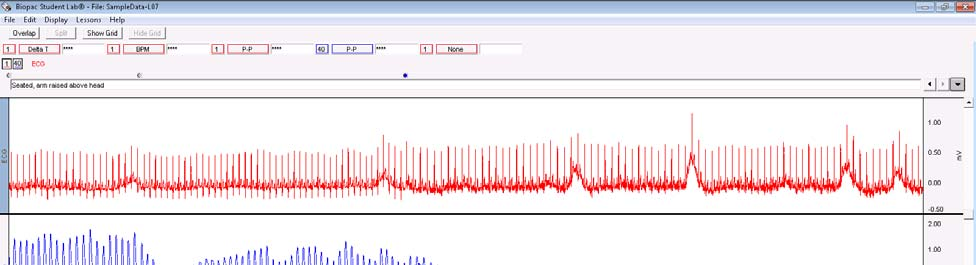
\includegraphics[width=0.8\textwidth]{../images/BIOPAC_5a.jpg}
		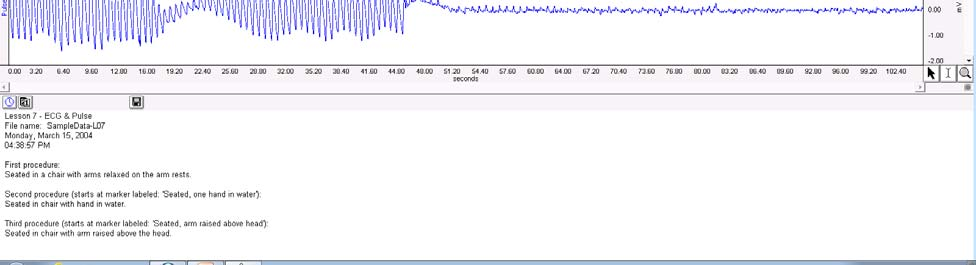
\includegraphics[width=0.8\textwidth]{../images/BIOPAC_5b.jpg}
		\centering
		\caption{L07 data file}
		\label{sample_data}
		\end{figure}
	
\end{enumerate}

\section*{Data Viewing Tools}
\begin{enumerate}
	\item The software consists of 2 main sections: data window (area with graphs) and journal window (area with text notes). Make sure you can find these on your computer.
	\item In this sample data, the data window contains two series of simultaneously recorded waveforms: an electrocardiogram (ECG) and a pulse. These waveforms depend on the physiological parameter measured and will change depending on the lesson recorded.
	\item Select the different markers (found above the marker bar in blue diamonds) and note from the markers what experiments were performed with this data set.
	\item Turn on and off channel 1 (ECG) and channel 40 (pulse). Remember that the channel boxes (found above the marker bar on the left) allow you to display or hide channels from view in order to concentrate or print out only the desired waveforms. The disabled channel will be hidden from. view, but can be turned back on at any time.
\end{enumerate}

\section*{Data Analysis Tools: Selection, I-beam, and Zoom Tools (
\includegraphics[width=0.08\textwidth]{../images/BIOPAC_selection.jpg})}
\begin{enumerate}
	\item Use the selection tool (arrow) to better select the section from 3 to 40 seconds: left click on the x-axis (seconds) to open the prompt seen in Fig. \ref{change_horiz} and hcange the scale range to display the desired data section.
	
		\begin{figure}[h]
		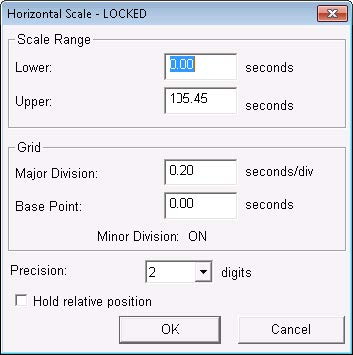
\includegraphics[width=0.6\textwidth]{../images/BIOPAC_8.jpg}
		\centering
		\caption{Changing the display for the horizontal scale}
		\label{change_horiz}
		\end{figure}
		
	\item Use the I-beam tool (looks like an I) to highlight different sections of the data. Notice that the measurement boxes (Delta T, BPM, P-P) will always display information corresponding to the highlighted region.
	\item Use the zoom tool (magnifying glass) to select an area of the data to be enlarged so as to make some analyses easier to perform. Use the zoom tool to display the waveform at approximately 12.6 seconds. Hold down the mouse button and drag the cursor downward and to the right so that the selected area includes approximately six spikes (see Fig. \ref{select_cycles}).
	
		\begin{figure}[h]
		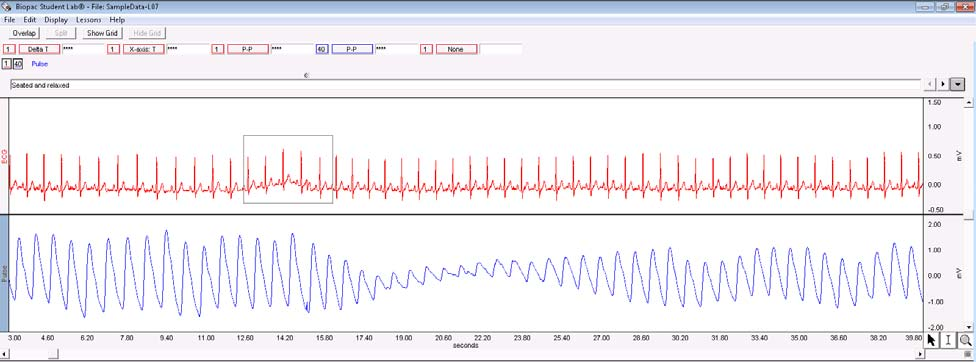
\includegraphics[width=0.8\textwidth]{../images/BIOPAC_9.jpg}
		\centering
		\caption{Selecting 6 cycles using the zoom tool}
		\label{select_cycles}
		\end{figure}
		
	\item Release the mouse button. Your data should not look like Fig. \ref{selected_cycles}. If you selected the wrong part of the data to magnify, pull down the Display menu and choose "Zoom Previous", then try again.
	
		\begin{figure}[h]
		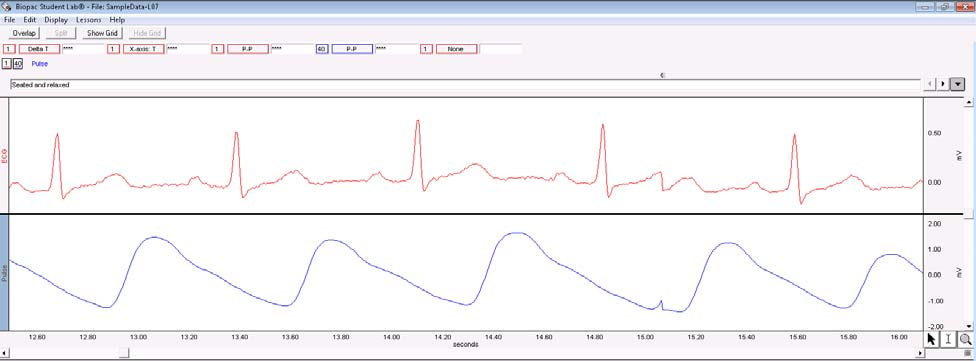
\includegraphics[width=0.8\textwidth]{../images/BIOPAC_10.jpg}
		\centering
		\caption{Selected region using zoom tool}
		\label{selected_cycles}
		\end{figure}	
\end{enumerate}

\section*{Channel Measurement Box}
\begin{enumerate}
	\item Right above the ECG recording channel, you will find the measurement boxes (Delta T, BPM, P-P). The first box indicates the \textit{recording channel} selected, the second box indicates the \textit{function or measurement} to be taken, and the third box contains the \textit{measurement value} (see Fig. \ref{meas_box}).
	
		\begin{figure}[h]
		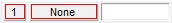
\includegraphics[width=0.4\textwidth]{../images/BIOPAC_16.jpg}
		\centering
		\caption{Channel measurement boxes}
		\label{meas_box}
		\end{figure}
		
	\item Using the first cycle (first beat), answer the following questions:
		\begin{enumerate}
			\item What is your measured value for delta T?
			\item What does delta T represent?
			\item What is your measured value for BPM?
			\item What does BPM represent?
			\item What are the "max" and "min" for the waveform on ECG?
			\item What are the "max" and "min" for the waveform on Pulse?
			\item What do the "max" and "min" values represent?
			\item Try out the options for "area", "P-P", "integral", "stdev", and two additional ones (see Table [add table at end] for available options and explanations). Explain in your own words what they are and the resulting value.
		\end{enumerate}
\end{enumerate}

\section*{Overlap/Split}
\begin{enumerate}
	\item These buttons allow you to toggle the display style between an oscilloscope and a chart recorder (see Fig. \ref{overlap_split})
	
		\begin{figure}[h]
		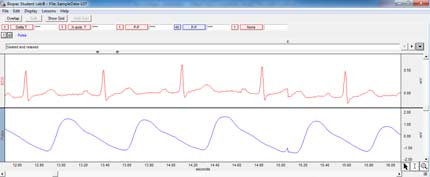
\includegraphics[width=0.8\textwidth]{../images/BIOPAC_11a.jpg}
		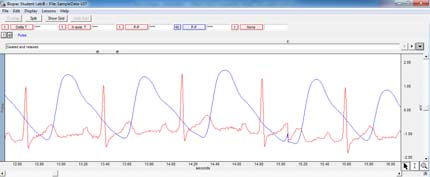
\includegraphics[width=0.8\textwidth]{../images/BIOPAC_11b.jpg}
		\centering
		\caption{Display types: split (top) and overlap (bottom)}
		\label{overlap_split}
		\end{figure}
	
	\item Click the overlap buttom to activate the type of display. Once the signals are overlapped, try to move each signal up and down separately for alignment.
		\begin{info}
			Select the channel box to select the appropriate channel to adjust.
		\end{info}
		
	\item Return the display type to split.
\end{enumerate}

\section*{Markers}
Markers are used to reference important events (and their associated locations) in the data. There are two types of markers:
\begin{itemize}
	\item 
\includegraphics[width=0.05\textwidth]{../images/BIOPAC_append_marker.jpg} \textit{Append markers}: These appear as a diamond above the marker text box and are blue when active. Append markers are automatically inserted when you begin each new recording segment and are marked with time data. Markers can also be manually entered during recording by pressing F9.
	
	\item 
\includegraphics[width=0.05\textwidth]{../images/BIOPAC_event_marker.jpg} \textit{Event markers}: These appear as inverted triangles below the marker text region and are yellow when active. You may add markers to your data after it has been recorded simply by clicking within the marker region using the selection tool. This new marker will then become the current active marker, and you may type in the marker text box.
\end{itemize}

\begin{figure}[h]
		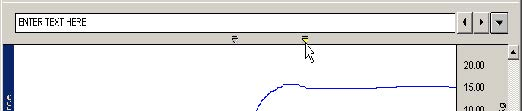
\includegraphics[width=0.8\textwidth]{../images/BIOPAC_12.jpg}
		\centering
		\caption{Marker tools are located in the top right, indicated by the arrows}
		\label{marker_tools}
		\end{figure}

Using the marker tools on the right edge of the marker region (Fig. \ref{marker_tools}), you may:
\begin{itemize}
	\item Change the active marker using the left and right pointing arrows
	\item Choose from the pop-up menu to find, clear, show, or import to journal certain or all markers (Fig. \ref{marker_menu}).
		\begin{figure}[h]
		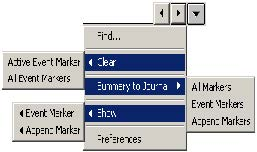
\includegraphics[width=0.6\textwidth]{../images/BIOPAC_13.jpg}
		\centering
		\caption{Marker tools pop-up menu}
		\label{marker_menu}
		\end{figure}
\end{itemize}

\begin{enumerate}
	\item How do you insert a marker while data are being recorded?
	\item How do you insert text for a marker?
	\item How do you insert an event marker after data have been recorded? Do this as practice.
\end{enumerate}

\end{document}
